\documentclass{standalone}


\begin{document}
	
	\subsection{Baselines}
	
	\begin{minted}{python}
def random_policy():
	"""
	Return a random walk of the agent, taking uniformly each possible action
	"""
	return [np.random.randint(0, 10) for i in range(5000)]		
		
def staticbest_policy(click_rates):
	"""
	Takes the action which maximises the score on that trajectory
	"""
	a = np.argmax(np.sum(click_rates, axis=0))
	return [a for i in range(5000)]
		
		
def opt_policy(click_rates):
	"""
	At each timestep takes the best action
	"""
	return np.argmax(click_rates, axis=1)
	\end{minted}
	
	\begin{figure}[H]
		\centering
		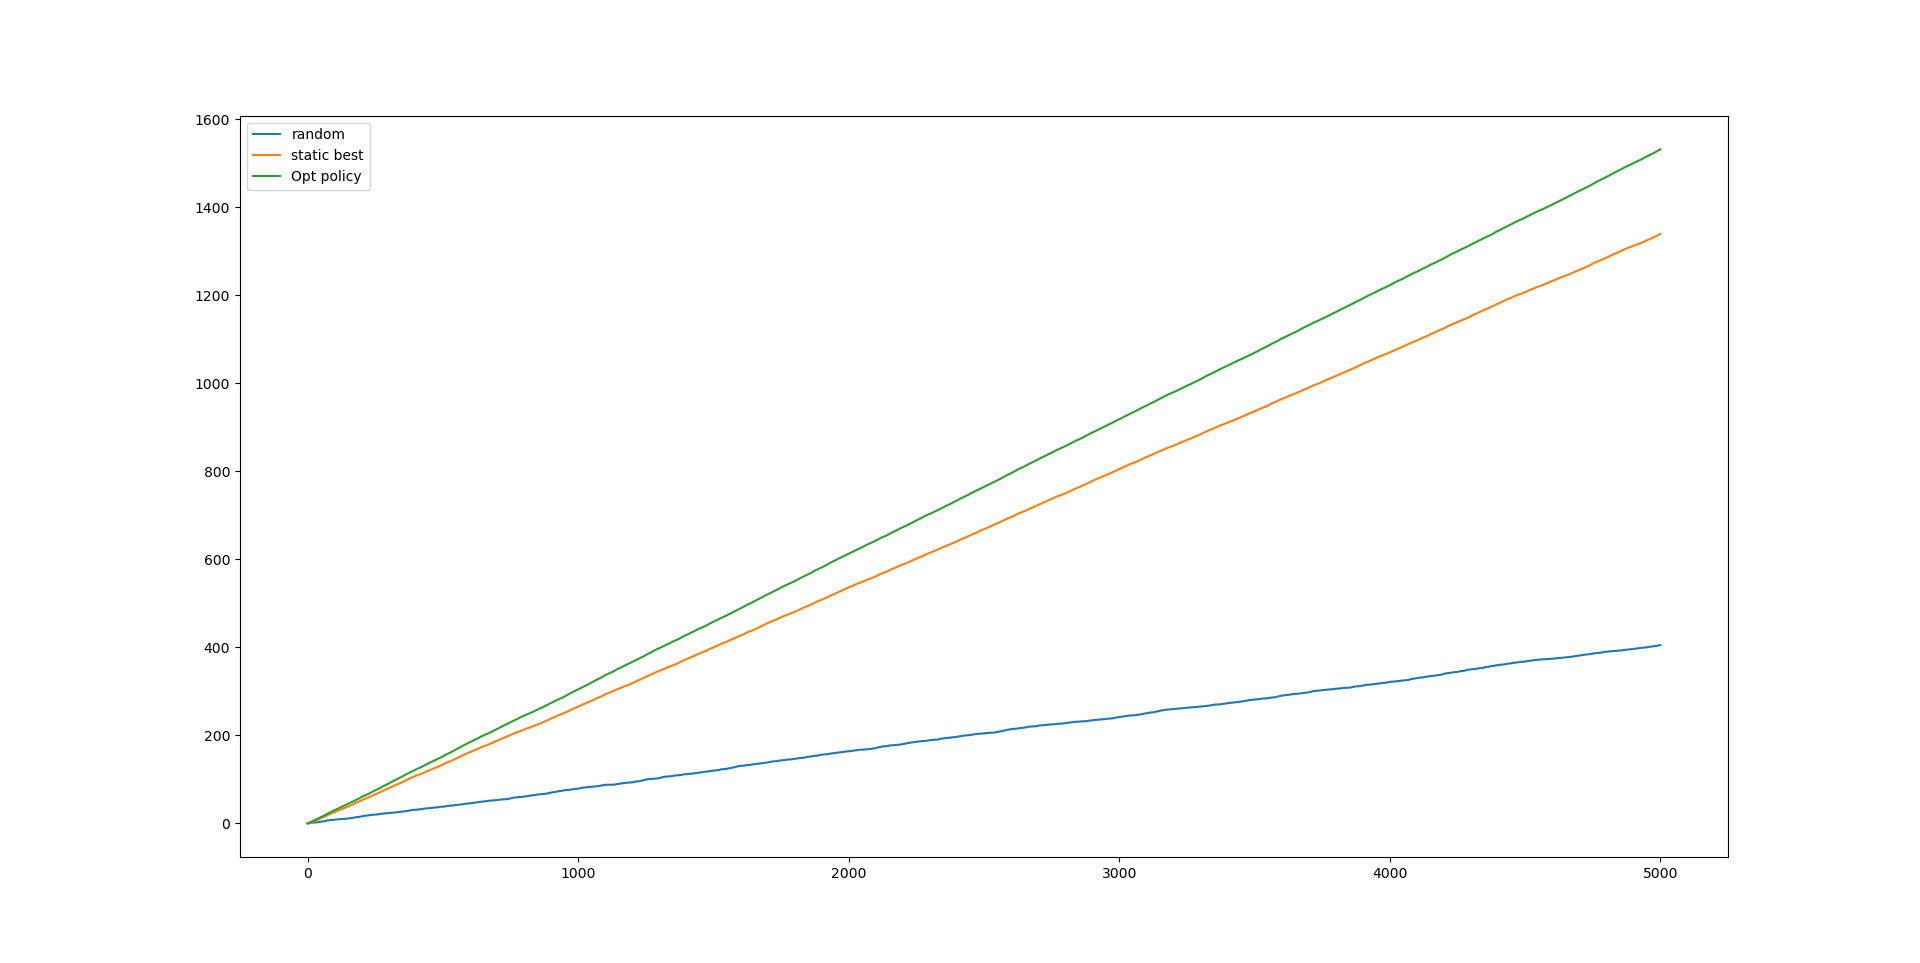
\includegraphics[scale=0.3]{img/baselines.png}
		\caption{Baselines -- agents omniscients}
	\end{figure}
	
	\subsection{UCB}
	
	\begin{minted}{python}
def upper_bound(t, N, mu):
	"""
	Computes the upper bound of the confidence interval of mean mu
	"""
	return mu + np.sqrt(2 * np.log(t) / N)

def ucb_policy(click_rates):
	"""
	Return the trajectory followed by the agent using ucb policy.
	"""
	
	# Cumulative reward got by each actions
	histo = np.array([click_rates[i][i] for i in range(10)])
	
	# Number of times we took each action
	counter = [1 for i in range(10)]

	# List of the taken action
	action_list = [i for i in range(10)]

	for t in range(10, 5000):
		action = np.argmax([upper_bound(t, counter[i], histo[i] / counter[i]) 
			for i in range(10)])
		counter[action] += 1
		histo[action] += click_rates[t][action]

		action_list.append(action)
	return action_list
	\end{minted}
	
		\begin{figure}[H]
		\centering
		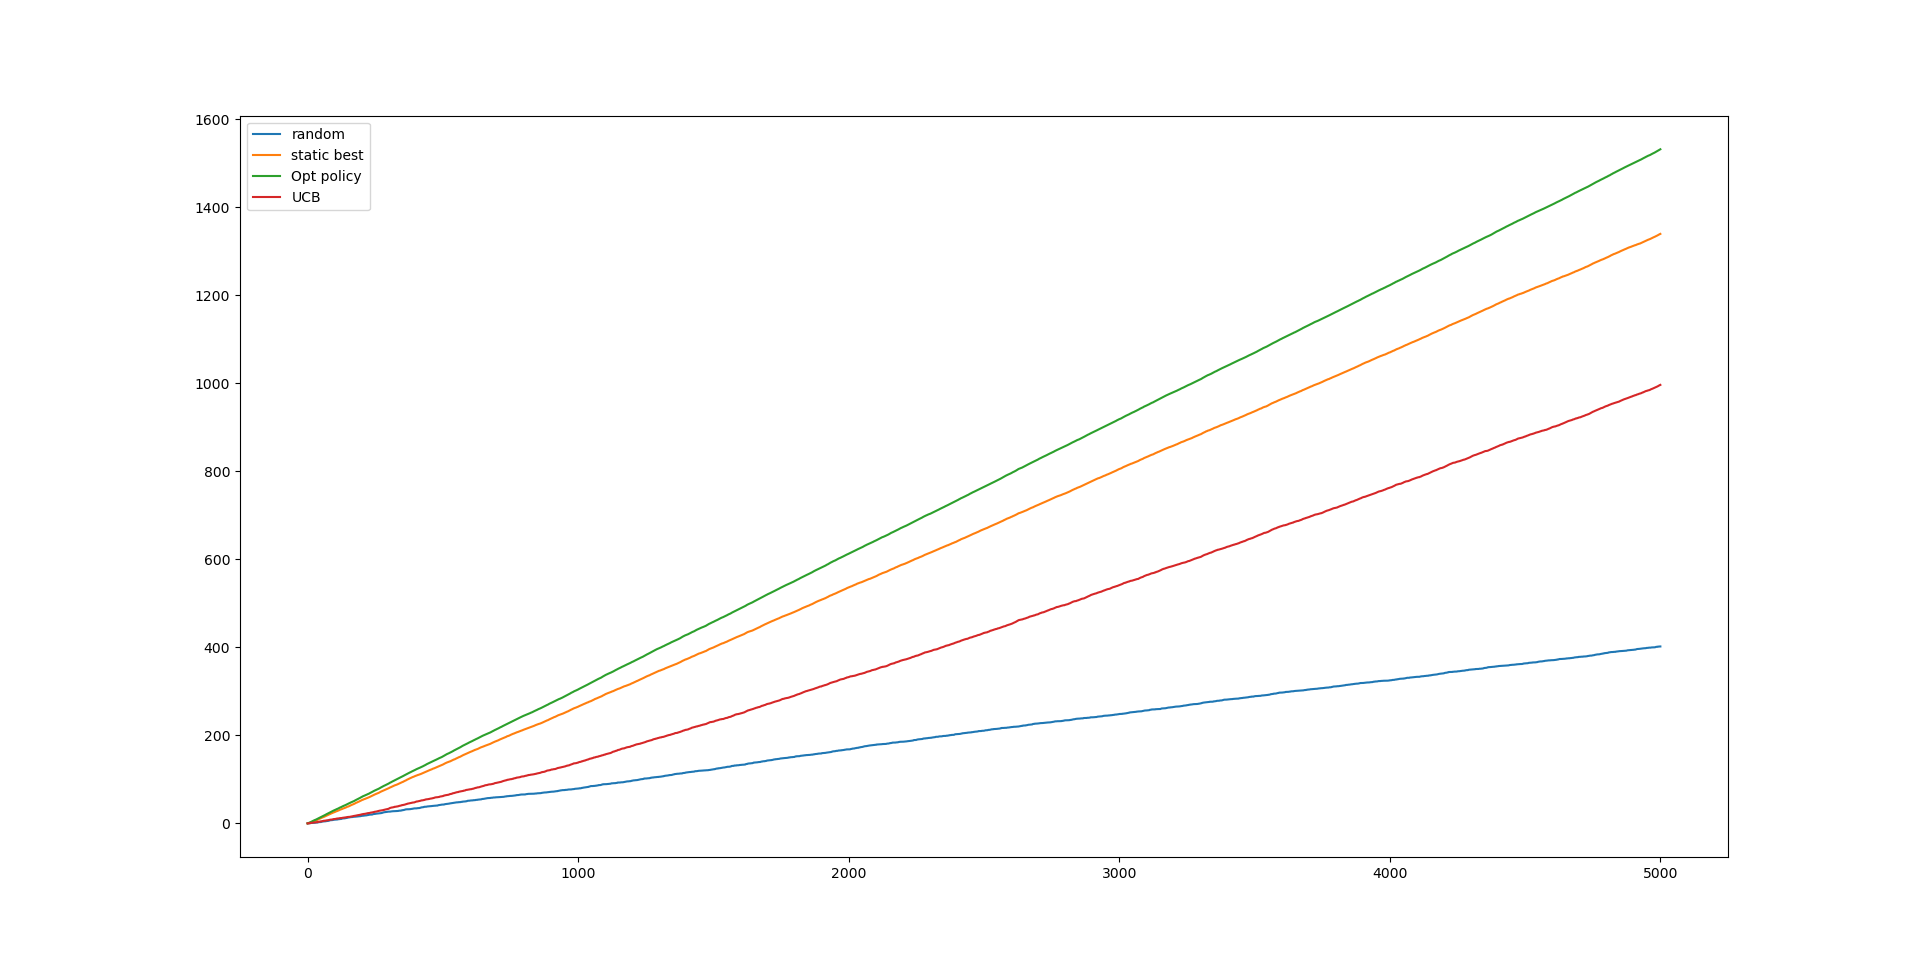
\includegraphics[scale=0.3]{img/ucb.png}
		\caption{Algorithme UCB VS Baselines}
	\end{figure}
	
	\subsection{LinUCB}
	
	\begin{minted}{python}
def linucb_policy(alpha, articles, click_rates):
	A = [np.identity(5, dtype=float) for i in range(10)]
	b = [np.zeros((5, 1), dtype=float) for i in range(10)]

	theta = [None for i in range(10)]
	pt = [None for i in range(10)]

	actions_list = []

	for t in range(0, 5000):
		for i in range(10):
			theta[i] = np.dot(np.linalg.inv(A[i]), b[i])

			pt[i] = (np.dot(np.transpose(theta[i]),  articles[t]) + alpha * np.sqrt(
			np.dot(
				np.dot(np.transpose(articles[t]),
						np.linalg.inv(A[i])),
				articles[t])))[0]

		at = np.argmax(pt)
		rt = click_rates[t][at]

		A[at] = A[at] + np.dot(np.transpose(articles[t]), articles[t])
		b[at] = b[at] + rt * articles[t]

		actions_list.append(at)

	return actions_list
	\end{minted}
	
	Dans figure suivante on compare \emph{Lin UCB} aux \emph{baselines} en faisant varier $\alpha$. En particulier on vérifie bien qu'un $\alpha$ bas correspond à une forte exploration (ici $\alpha = 0.01$ donne des résultats proches de l'aléatoire) tandis que des valeurs plus importantes permettent un meilleur compromis exploration-exploitation.
	
	\begin{figure}[H]

			\centering
			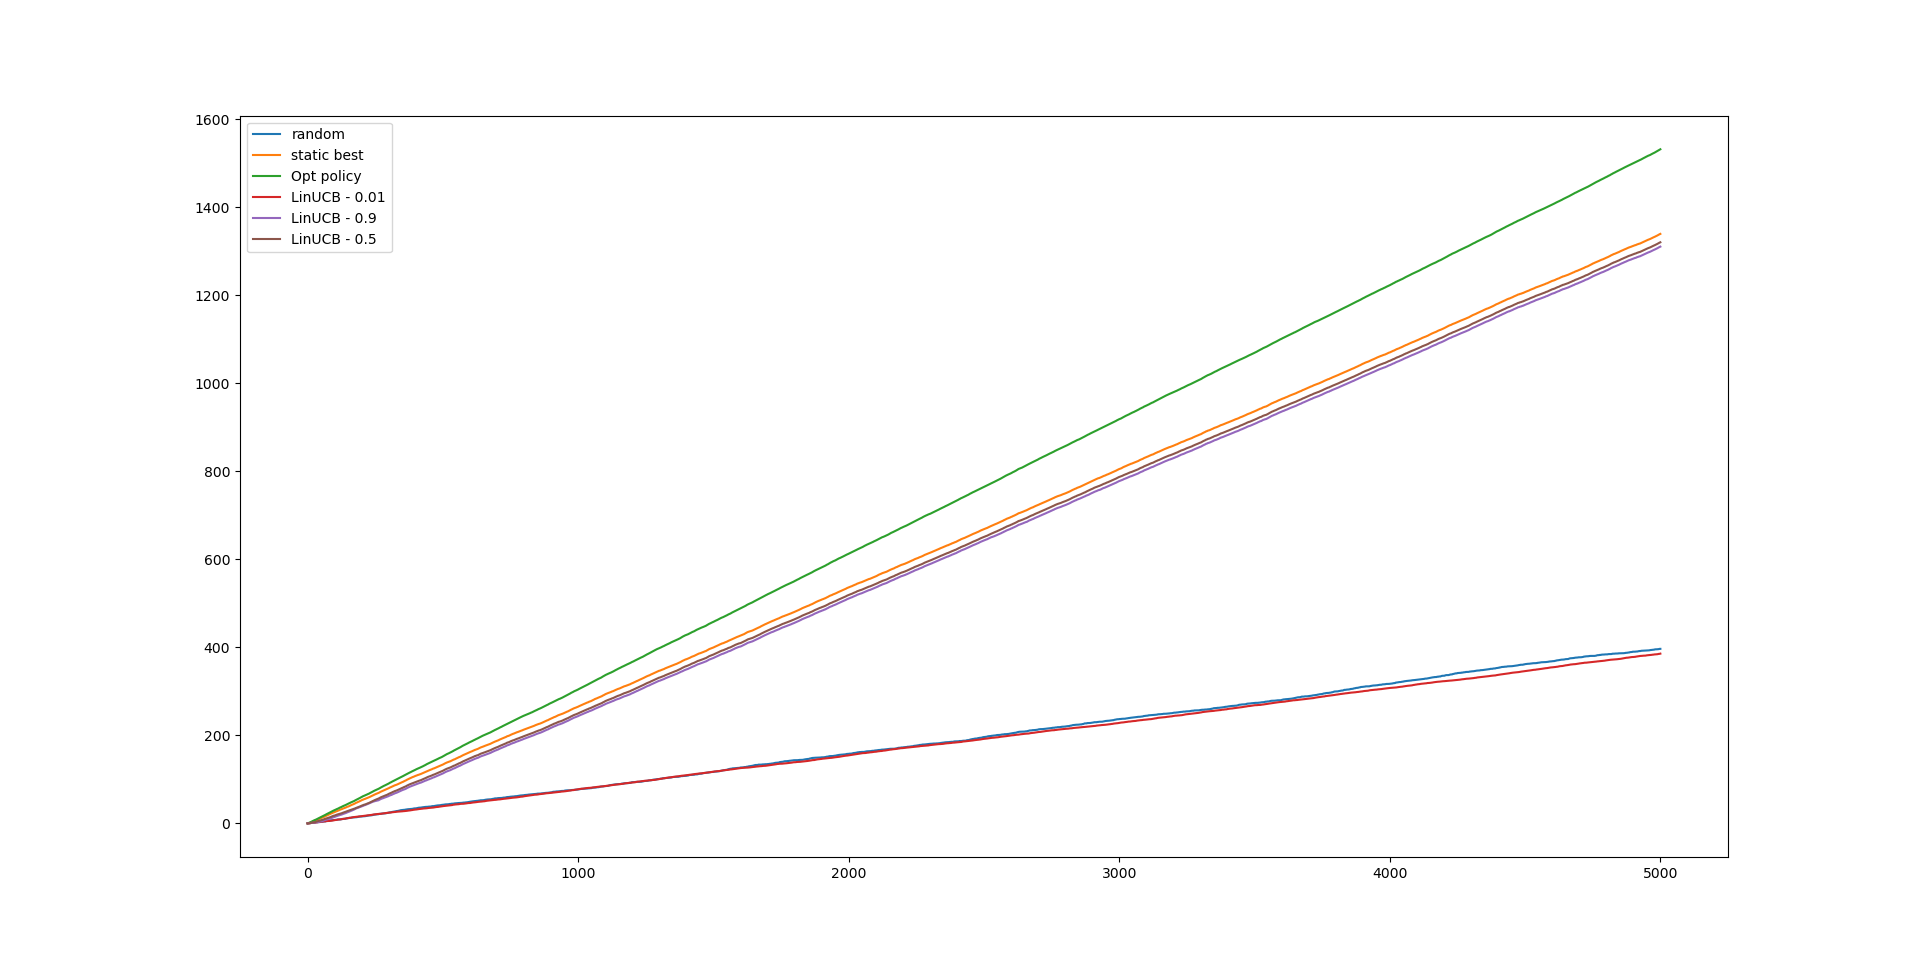
\includegraphics[scale=0.3]{img/lin_ucb.png}
			\caption{Algorithme LinUCB VS Baselines}

	\end{figure}

Par ailleurs, on observe bien que \emph{lin UCB} est clairement meilleur que \emph{UCB}. En effet, en utilisant le contexte pour prendre des décisions plus averties. 

\begin{figure}[H]
	\centering
	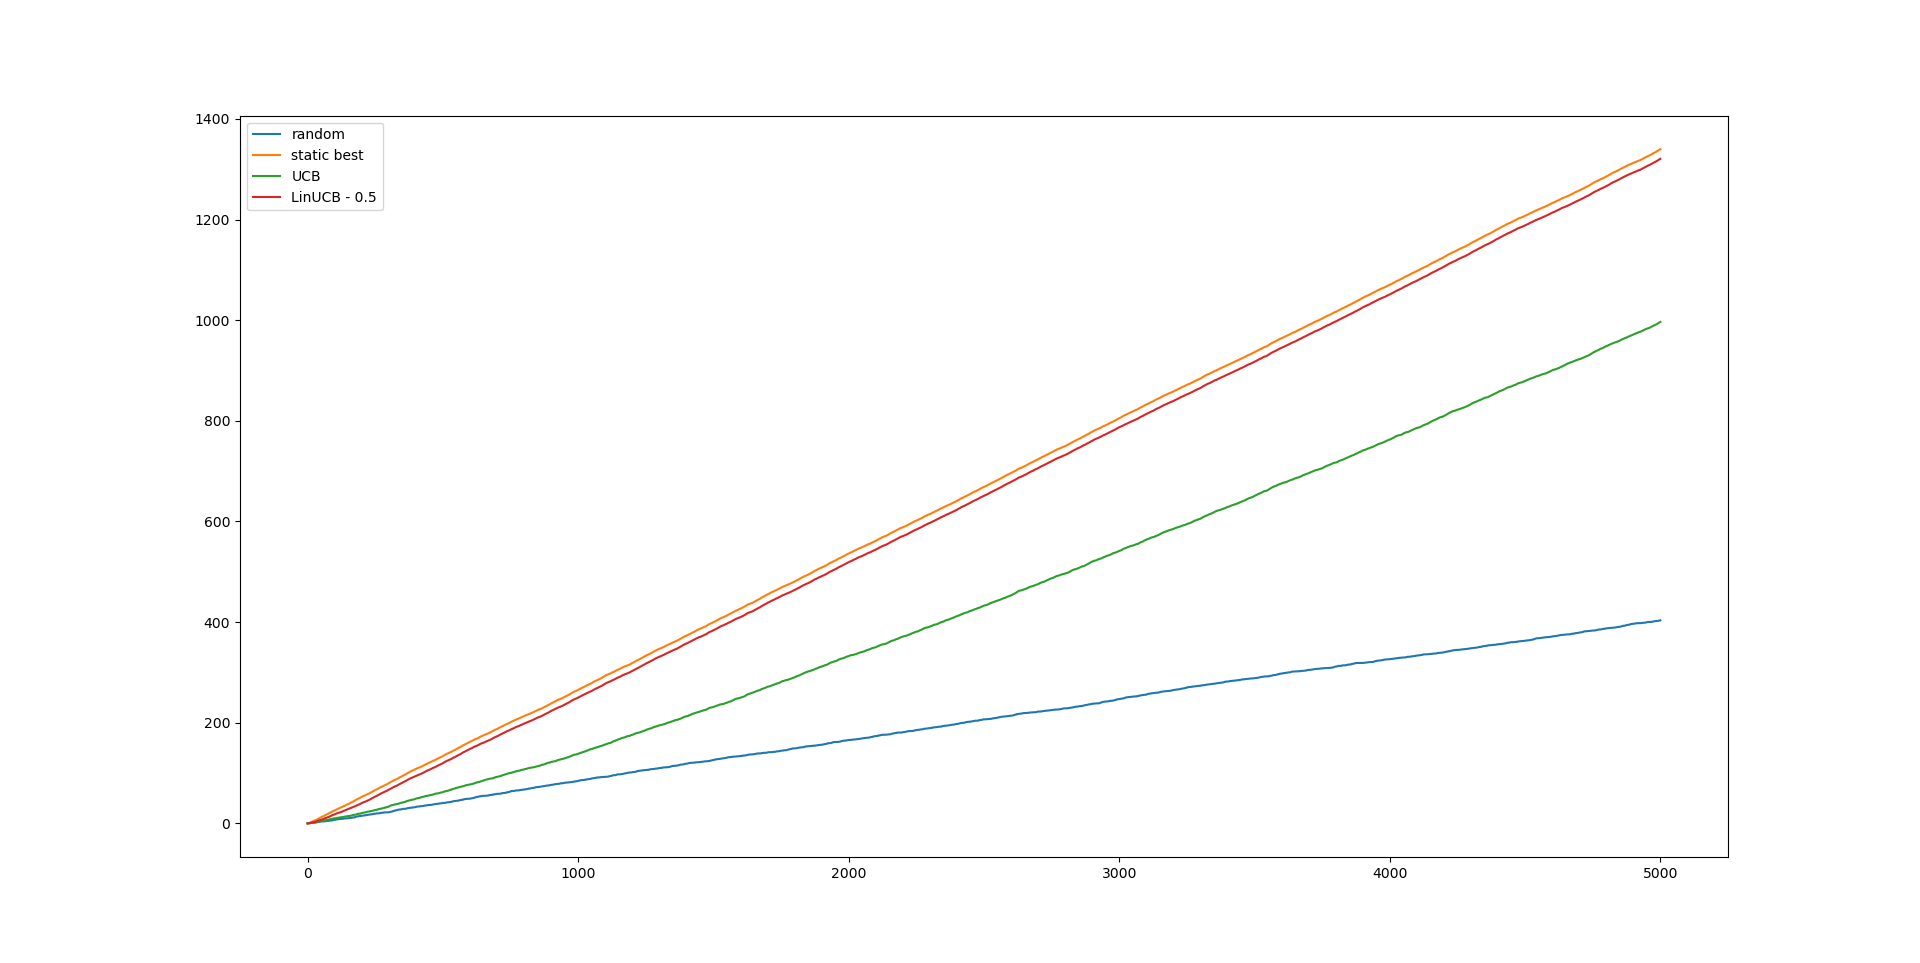
\includegraphics[scale=0.3]{img/linucb_ucb.png}
	\caption{Algorithme LinUCB VS UCB}
\end{figure}


	
\end{document}
